\documentclass[a4paper]{article}
\usepackage[margin=0.6in]{geometry}

\usepackage[utf8]{inputenc}
\usepackage{indentfirst}
\usepackage{graphicx}

\usepackage{hyperref}

\title{Securitatea Informației - Tema 3\\
        Atacul SYN Flooding}
\author{Oloieri Alexandru IIIA2}
\date{Ianuarie 2021}

\begin{document}

\maketitle

\section{Modul de funcționare a atacului SYN Flooding}

Un atac de tipul \textbf{denial-of-service (DoS attack)} are loc atunci când un atacator suprasolicită o resursă cu cereri false, ea nemaifiind disponibilă celorlalți utilizatori (adică serverul nu mai poate răspunde cererilor reale).

Atacul \textbf{SYN Flood} este un tip de atac \textbf{DoS} în care adversarul se folosește de modul în care se realizează conexiunile TCP pentru a consuma suficiente resurse de pe server astfel încât acesta să nu mai poată răspundă la cererile utilizatorilor reali pe care le primește.

O conexiune normală TCP se realizează în 3 pași (TCP 3-Way Handshake):

\begin{enumerate}
    \item Clientul trimite serverului un segment TCP ce conține o valoare numită \textbf{SYN} (Synchronize Sequence Number).
    
    \item Serverul răspunde cu un pachet ce conține bitul SYN-ACK setat și de asemenea alte 2 valori: SYN-ul serverului și ACK (SYN-ul primit de la client + 1).
    
    \item Clientul trimite serverului ACK, o valoare egală cu SYN-ul primit de la server + 1. După acest pas conexiunea este stabilită.
    
\end{enumerate}

Un atacator poate realiza un atac \textbf{DoS} în felul următor: va trimite o cantitate mare de cereri SYN către server (la un anumit port), fără a încheia însă conexiunile. Serverul va reține pentru un anumit timp ce conexiuni au venit (și n-au fost însă închise) într-o coadă, iar când aceasta se umple el nu va mai putea răspunde altor cereri de conectare (care pot veni și de la clienți reali). Atacatorul va utiliza de cele mai multe ori și o tehnică numită \textbf{IP Spoofing}, care presupune crearea pachetelor cu adrese IP false, astfel încât serverul să nu știe dacă pachetul vine de la un client real sau nu, și deci să-i fie imposibil să le ignore.

\section{Mediul de lucru}

Vom simula atacul pe o rețea formata din 3 mașini Linux (Ubuntu 16.04), configurarea mediului de lucru fiind realizată conform indicațiilor de pe pagina domnului profesor Emanuel Onica (\href{https://profs.info.uaic.ro/~eonica/isec/lab10.html}{aici}):

\begin{center}
    \begin{tabular}{|c|c|c|}
         \hline
         Numele mașinii & Adresa IP & Rol \\
         $ VM_1 $ & 192.168.0.1 & Observator \\
         $ VM_2 $ & 192.168.0.2 & Atacator \\
         $ VM_3 $ & 192.168.0.3 & Victima \\
         \hline
    \end{tabular}
\end{center}

În plus, ne vom folosi de următoarele:

\begin{enumerate}
    \item Aplicația \textbf{wireshark}, care va fi folosită pe mașina $ VM_1 $ pentru a monitoriza traficul în rețeaua locală.

    \item Comanda \textbf{hping3} pentru implementarea atacului propriu-zis.

    \item Comenzi ca \textbf{sysctl} sau \textbf{netstat} pentru verificarea dimensiunii cozii unde sunt plasate cererile de conectare sau pentru a vedea câte conexiuni se află în curs de stabilire.

    \item Comanda \textbf{service vsftpd start} pentru a porni un server FTP.

\end{enumerate}

\section{Descrierea modului în care vom realiza atacul}

\begin{enumerate}
    \item Pe mașina $ VM_3 $ vom porni un server FTP, care va aștepta cereri de conectare pe portul 21. (Ne vom conecta la serverul FTP de pe mașina $ VM_1 $ pentru a vedea că într-adevăr conexiunile sunt posibile înainte de atac)
    
    \item Vom porni un atac SYN Flood de pe mașina $ VM_2 $. Rulând comanda \textbf{netstat -tna} pe $ VM_3 $ ar trebui să vedem o mulțime de conexiuni aflate în starea \textbf{SYN\_RECV} și de asemenea ar trebui să vedem și pachetele pe mașina $ VM_1 $ în aplicația \textbf{wireshark}.
    
    \item Vom încerca din nou să ne conectăm la serverul FTP de pe mașina $ VM_1 $, însă de această dată nu vom reuși (cel mai probabil vom primi mesajul \textbf{Connection timed out}).
    
    \item Vom opri atacul de pe mașina $ VM_2 $ iar acum ne vom putea conecta cu succes la serverul FTP (iar conexiunea realizată cu succes va putea fi observată și în urma rulării comenzii \textbf{netstat -tna} pe mașina $ VM_3 $).

\end{enumerate}

\section{Realizarea atacului}

\begin{enumerate}
    \item Pornim serverul FTP pe mașina $ VM_3 $ (\textbf{sudo service vsftpd start}), și ne asigurăm că portul 21 acceptă conexiuni cu comanda \textbf{netstat -tna}.
    
    \begin{center}
        \hspace*{-1.8cm}                                           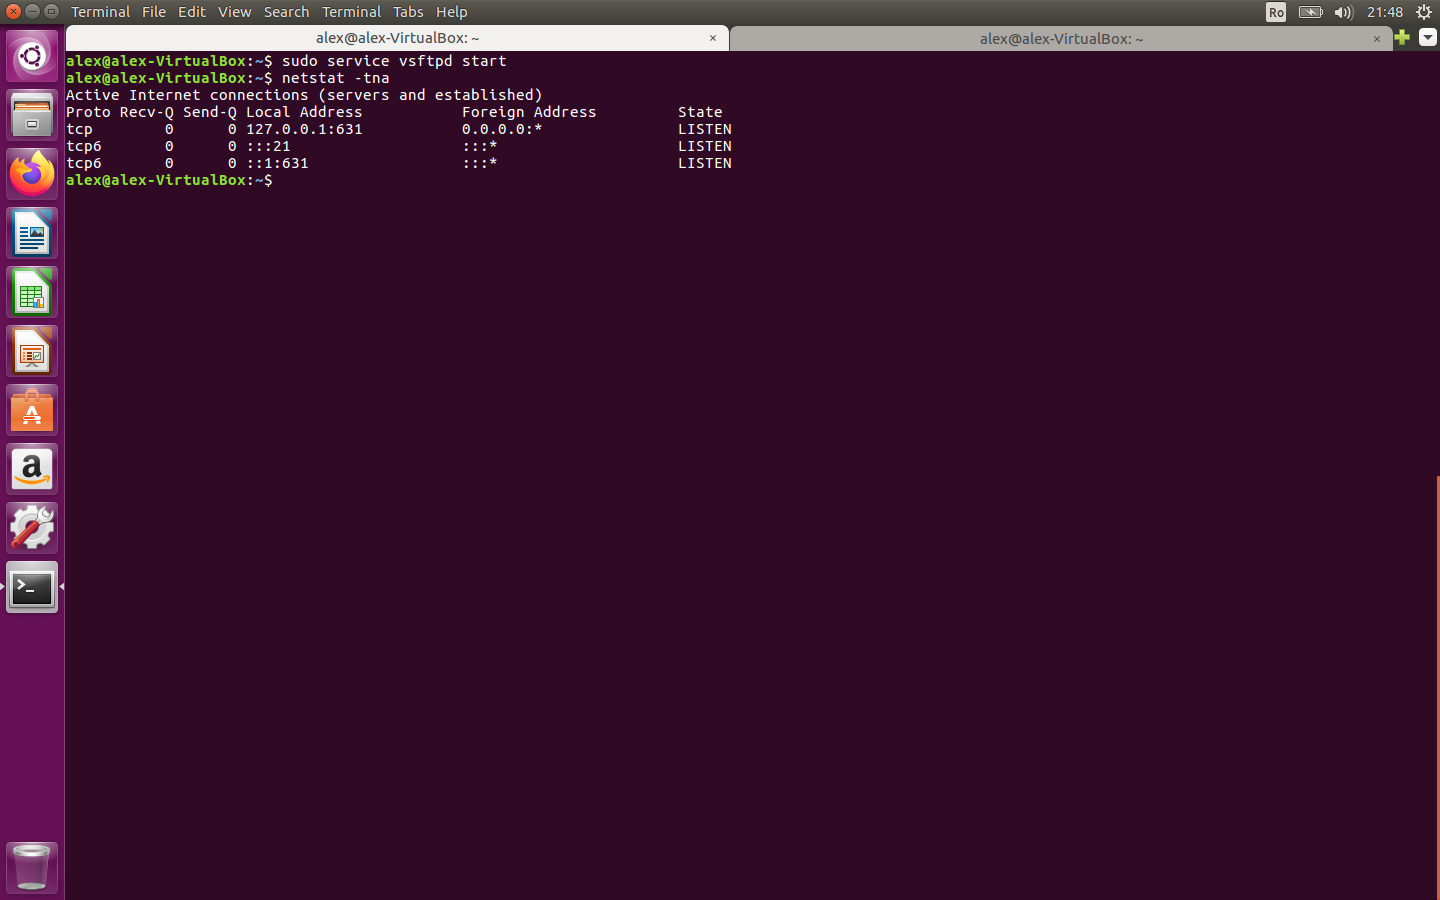
\includegraphics[scale=0.64]{"./img/pas1.png"}       
    \end{center}
    
    \item Ne conectăm la serverul FTP de pe mașina $ VM_1 $ pentru a vedea că într-adevăr serverul rulează: $ ftp 192.168.0.3 $, iar apoi introducem credențialele.
    
    \begin{center}
        \hspace*{-1.8cm}                                           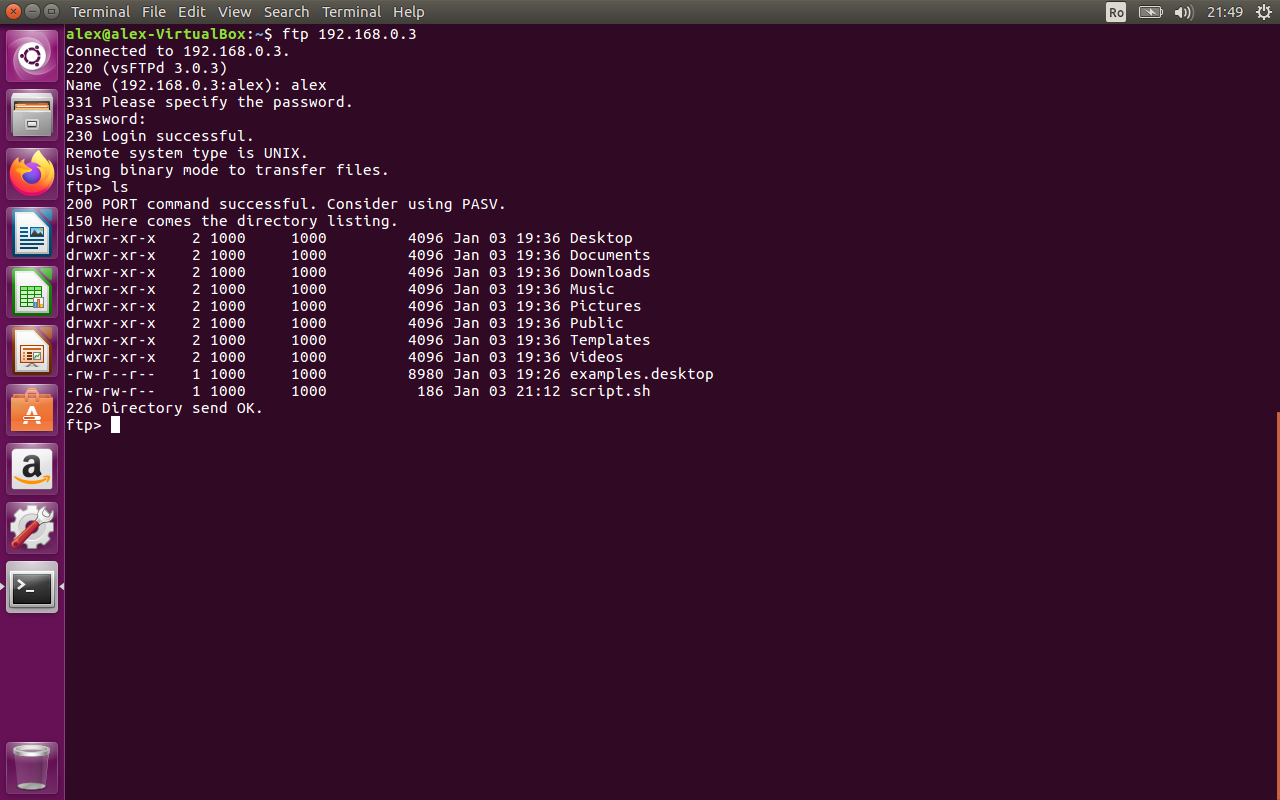
\includegraphics[scale=0.64]{"./img/pas2.png"}       
    \end{center}
    
    \item Pornim atacul \textbf{SYN\_FLOOD}: rulăm următoarea comandă pe mașina $ VM_2 $: \textbf{sudo hping3 -c 15000 -d 120 -S -w 64 -p 21 --flood --rand-source 192.168.0.3}. Semnificația parametrilor: 15000 de pachete (\textbf{-c 15000}) de dimensiune 120 de bytes (\textbf{-d 120}) vor fi trimise cât de repede posibil (\textbf{--flood}); pachetele vor avea SYN Flag (\textbf{-S}) activat,  dimensiunea TCP windows size va fi 64 (\textbf{-w 64}), iar adresele ip vor fi generate random (\textbf{--rand-source}). Toate aceste pachete vor fi trimise mașinii având adresa IP \textbf{192.168.0.3} ($ VM_3 $), la portul \textbf{21} (unde așteaptă conexiuni serverul FTP).
    
    \begin{center}
        \hspace*{-1.8cm}                                           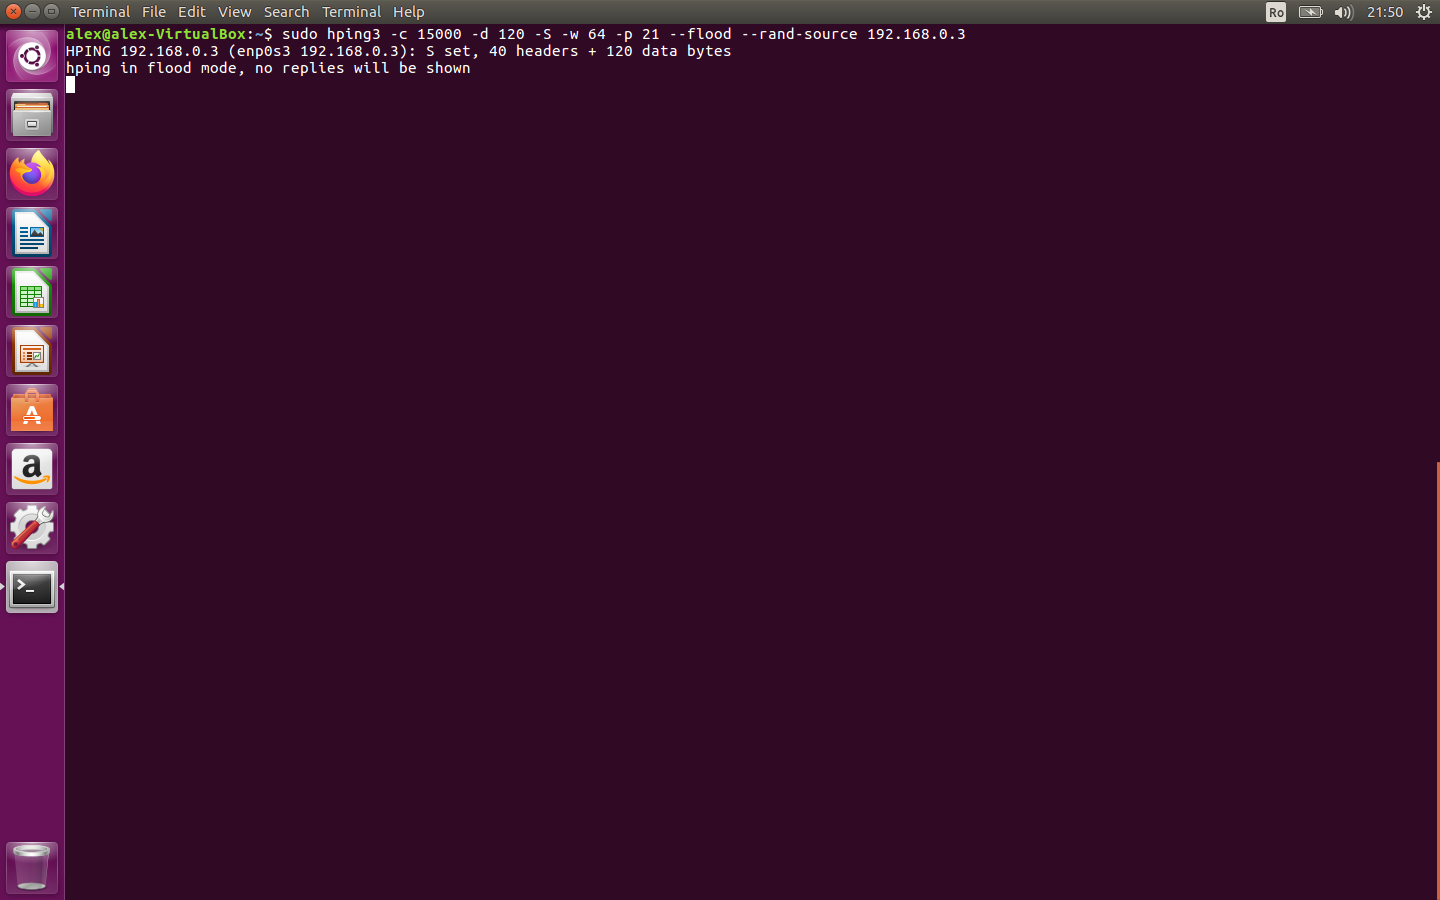
\includegraphics[scale=0.56]{"./img/pas3.png"}       
    \end{center}
    
    \item Verificăm că pe mașina $ VM_3 $ sunt multe conexiuni aflate în starea \textbf{SYN\_RECV} folosind din nou comanda \textbf{netstat -tna}.
    
    \begin{center}
        \hspace*{-1.8cm}                                           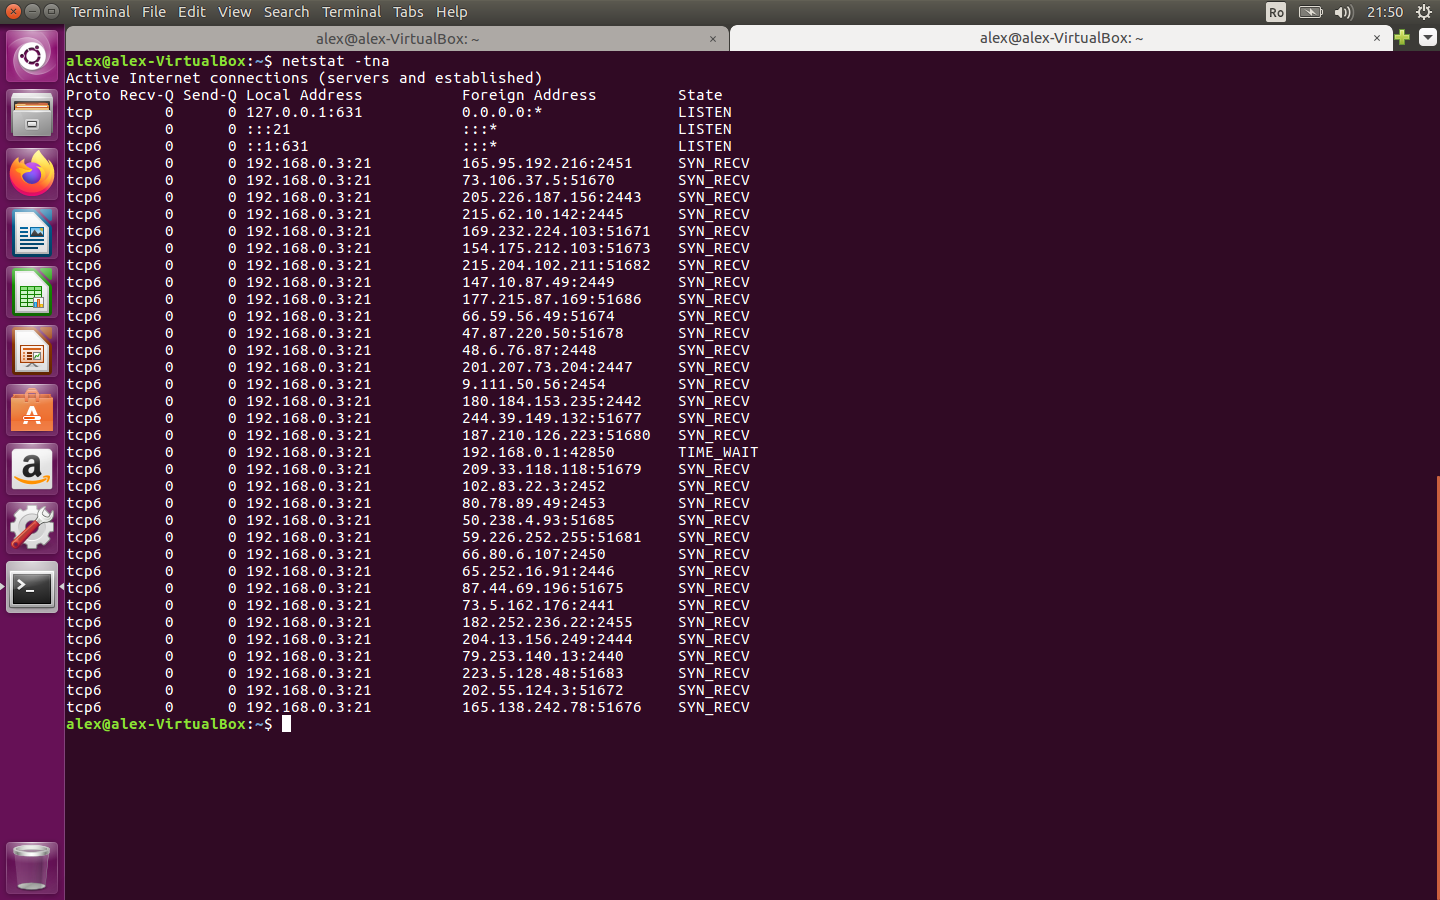
\includegraphics[scale=0.56]{"./img/pas4.png"}       
    \end{center}
    
    \item Vizualizăm pachetele în aplicația \textbf{wireshark} pe mașina $ VM_1 $.
    
    \begin{center}
        \hspace*{-1.8cm}                                           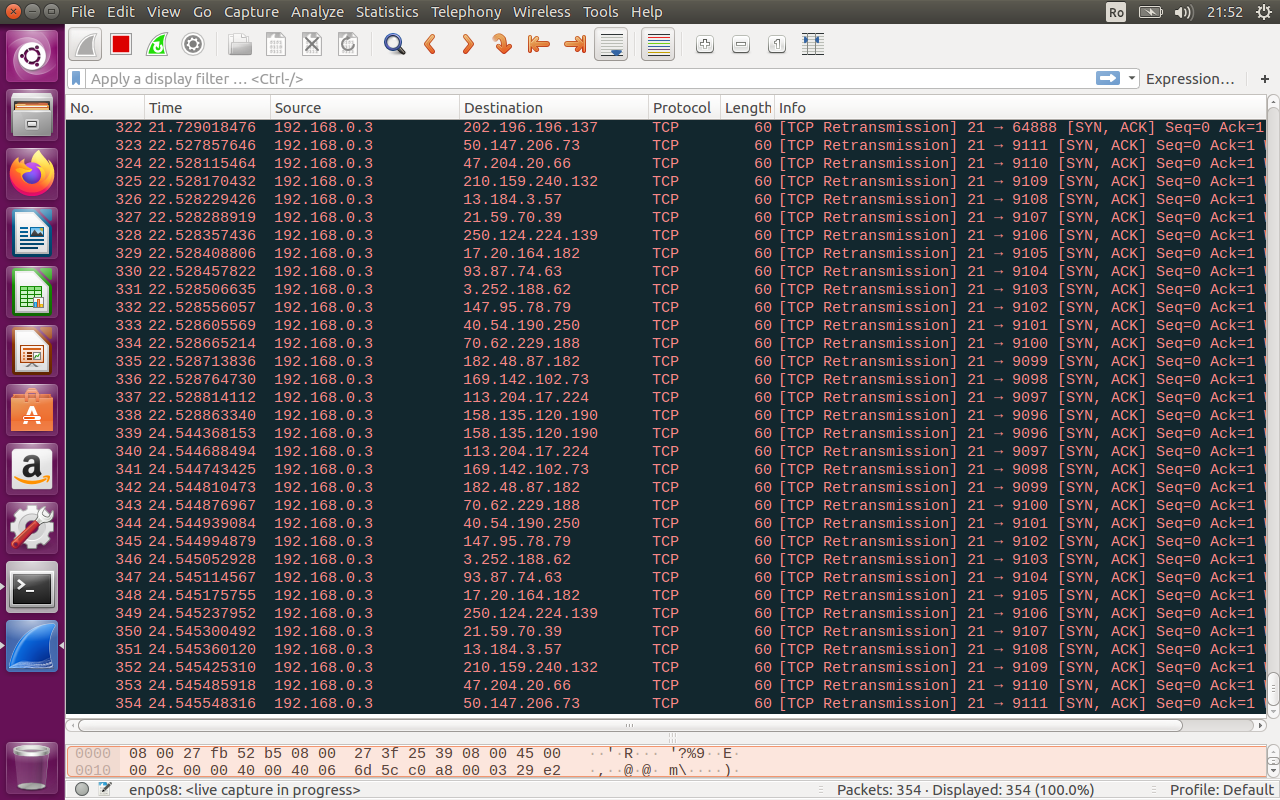
\includegraphics[scale=0.64]{"./img/pas6.png"}       
    \end{center}
    
    \item Încercăm să ne conectăm din nou la serverul FTP de pe mașina $ VM_1 $, însă de această dată nu vom reuși.
    
    \begin{center}
        \hspace*{-1.8cm}                                          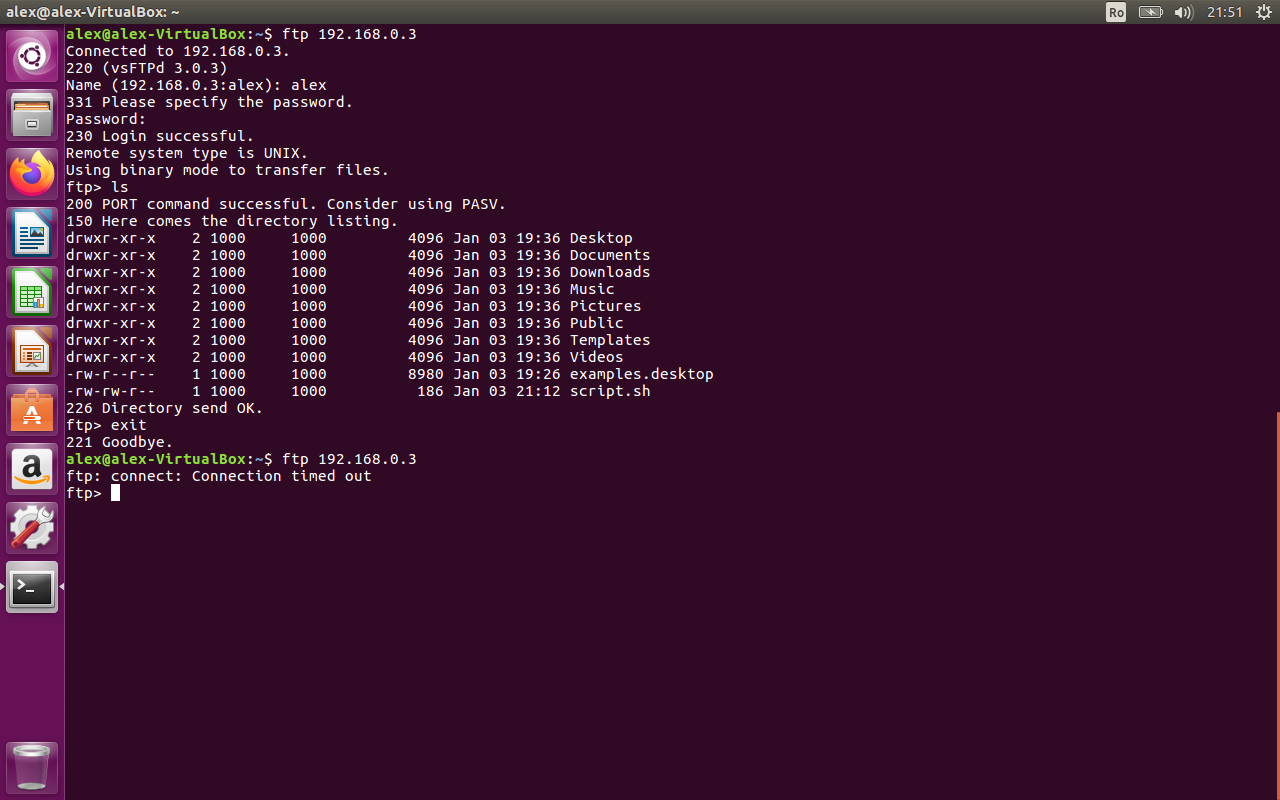
\includegraphics[scale=0.64]{"./img/pas5.png"}       
    \end{center}
    
    \item Oprim atacul (\textbf{CTRL + C}) de pe mașina $ VM_2 $, iar acum ne putea conecta din nou la serverul FTP de pe mașina $ VM_1 $.
    
    \begin{center}
        \hspace*{-1.8cm}                                          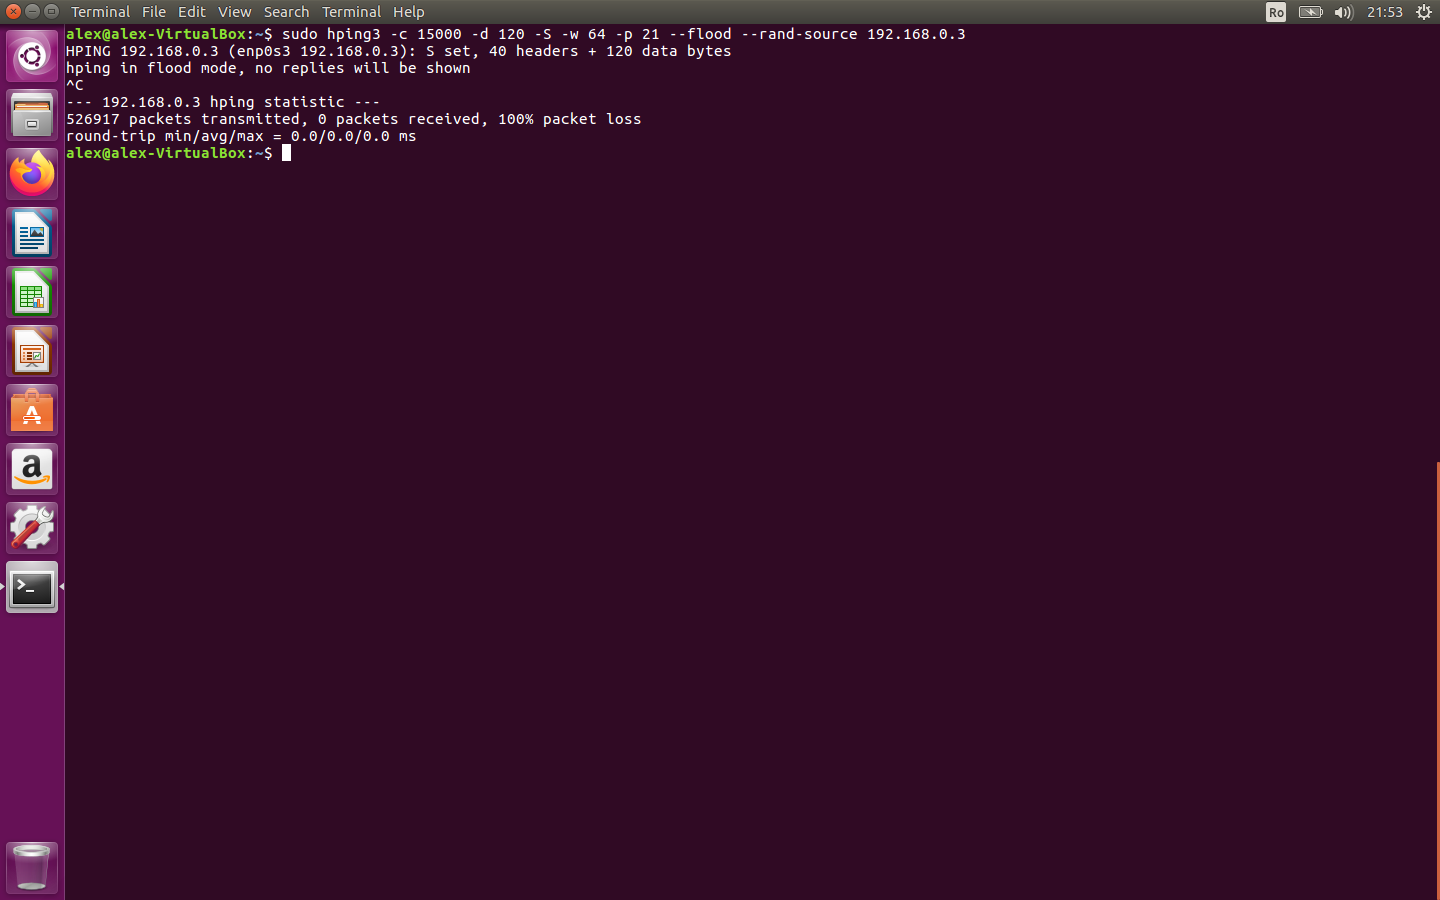
\includegraphics[scale=0.64]{"./img/pas7.png"}       
    \end{center}
    
    \begin{center}
        \hspace*{-1.8cm}                                          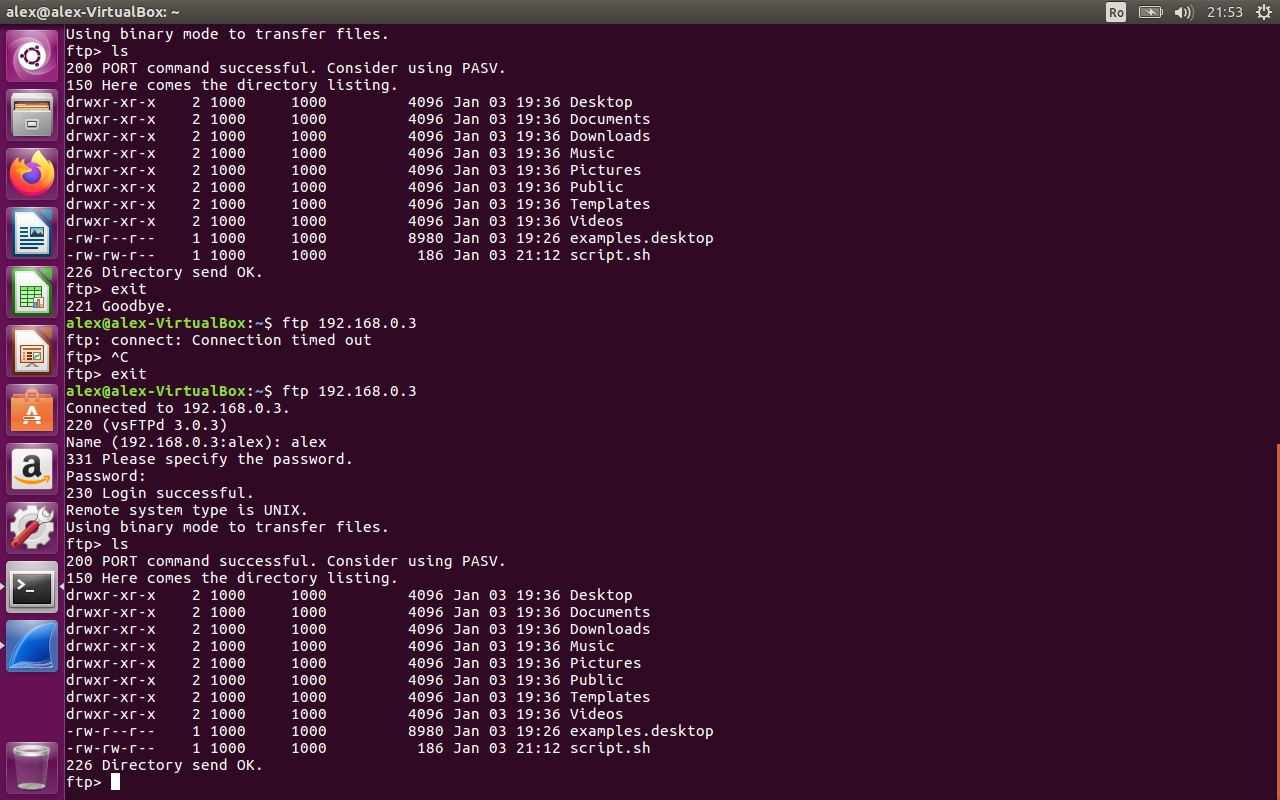
\includegraphics[scale=0.64]{"./img/pas8.png"}       
    \end{center}
    
\end{enumerate}

Timpul de execuție: după pornirea atacului durează câteva secunde până când serverul devine inaccesibil clienților reali.

\section{Moduri de a preveni atacul}

\begin{enumerate}
    \item Folosirea unui server/firewall intermediar care va redirecta numai un număr limitat de conexiuni către serverul principal (conexiuni care au fost deja verificate ca fiind valide, de la utilizatori reali): \href{https://www.youtube.com/watch?v=nYPFH1ZAlck&ab_channel=CBTNuggets}{mai multe detalii aici}.

    \item \textbf{SYN Cookie} e o tehnică folosită pentru prevenirea atacurilor \textbf{SYN\_FLOOD}. În loc să rețină conexiunile, se codifică numărul trimis în răspunsul SYN+ACK. Dacă serverul primește un răspuns cu un ACK incrementat, acesta știe să reconstruiască valoarea SYN și conexiunea continuă în mod normal. Pentru activarea/dezactivarea lor se poate folosi comanda \textbf{sudo sysctl net.ipv4.tcp\_syncookies = 1/0}.
    
\end{enumerate}

\begin{thebibliography}{9}
		
	\bibitem{b1}
	    How to perform a TCP SYN Flood attack
	    \url{http://www.firewall.cx/general-topics-reviews/network-protocol-analyzers/1224-performing-tcp-syn-flood-attack-and-detecting-it-with-wireshark.html}

    \bibitem{b2}
        \url{https://profs.info.uaic.ro/~eonica/isec/lab10.html}
    
    \bibitem{b3}
        \url{https://profs.info.uaic.ro/~eonica/isec/lab12.html}

    \bibitem{b4}
        SYN cookies
        \url{https://en.wikipedia.org/wiki/SYN_cookies}

    \bibitem{b5}
        TCP 3-Way Handshake
        \url{https://www.geeksforgeeks.org/tcp-3-way-handshake-process/}

    \bibitem{b6}
        SYN Flood
        \url{https://en.wikipedia.org/wiki/SYN_flood}

\end{thebibliography}

\end{document}
